\cleardoublestylepage{common}

\section{CWA指导的SMD框架:CWA-SMD}

将CWA方法与SMD方法结合起来的最为直接的方法便为CWA指导SMD:即通过CWA演化后得到的一系列期望值作为SMD方法的截断。我们从初始的波函数进行维格纳变换得到相空间分布,
\begin{equation}
  \mathcal{W} \left[ \psi \right] (\boldsymbol{X}, \boldsymbol{P}) = \left(\frac{1}{2\pi \hbar}\right)^n \int \psi(\boldsymbol{X}-\boldsymbol{Y}/2) \psi(\boldsymbol{X} + \boldsymbol{Y}/2) e^{i \boldsymbol{P} \cdot \boldsymbol{Y} / \hbar} \, \mathrm{d}\boldsymbol{Y} 
\end{equation}
其中$\boldsymbol{X}, \, \boldsymbol{P}$分别代表体系的位移自由度和平移自由度,并以此相空间分布为基础得到的任意可观察量的期望值必定是精确的。同时,将其进行离散化处理,对初始波函数$\psi_0(\boldsymbol{X})$及其对应相空间分布$ \Gamma_0(\boldsymbol{X}, \boldsymbol{P}) = \mathcal{W}\left[ \psi_0(\boldsymbol{X}) \right] $, 做近似
\begin{equation}
  \Gamma_0 (\boldsymbol{X}, \boldsymbol{P}) \sim \sum_{i,j} \Gamma_{ij}'(\boldsymbol{X}, \boldsymbol{P}) = \sum c_{ij} \delta(\boldsymbol{X} - \prescript{0}{}{\boldsymbol{q}_i}) \delta(\boldsymbol{P} - \prescript{0}{}{\boldsymbol{p}_j})
\end{equation}
其中$\left\{ \prescript{0}{}{\boldsymbol{q}_i}, \prescript{0}{}{\boldsymbol{p}_j} \right\} $ 为相空间某区域均匀分布的格点,以及
\begin{equation}
  c_{ij} = \int \Gamma_0(\boldsymbol{X}, \boldsymbol{P}) \delta(\boldsymbol{X} - \prescript{0}{}{\boldsymbol{q}_i}) \delta(\boldsymbol{P} - \prescript{0}{}{\boldsymbol{p}_j}) \, \mathrm{d}\boldsymbol{X}\mathrm{d}\boldsymbol{P}
\end{equation}
演化利用泊松括号来实现,
\begin{equation}
\frac{\mathrm{d}}{\mathrm{d}t} \Gamma'_{ij}(\boldsymbol{X}, \boldsymbol{P})
\begin{cases}
	\frac{\mathrm{d} c_{ij}}{\mathrm{d} t} = 0 , \\
	\frac{\mathrm{d} \boldsymbol{q}_i}{\mathrm{d} t} = \frac{\boldsymbol{p}_j}{m} , \\
	\frac{\mathrm{d} \boldsymbol{p}_j}{\mathrm{d} t} = - \frac{\partial V(\boldsymbol{X})}{\partial \boldsymbol{X}}\bigg|_{\boldsymbol{X} = \boldsymbol{q_i}}
\end{cases}
\end{equation}
该部分即为CWA的演化方法,同时不受SMD方法的干涉。对于SMD部分,准备$\boldsymbol{X}$与$\boldsymbol{P}$的幂函数$\{P_i(\boldsymbol{X},\boldsymbol{P})\}$或其他存在迭代形式的函数形式作为可观察量组,构建演化方程
\begin{equation}
\frac{\mathrm{d}}{\mathrm{d} t} \langle P_i(\boldsymbol{X},\boldsymbol{P}) \rangle = \langle \{\{P_i(\boldsymbol{X},\boldsymbol{P}), H\}\} \rangle
\end{equation}
其中 $\{\{ *, * \}\}$为磨雅括号,定义为
 \begin{equation}
	 \{\{f, g\}\}=\frac{2}{\hbar} f \sin \left[\frac{\hbar}{2}\left(\sum_{i} \overleftarrow{\partial}_{q_{i}} \overrightarrow{\partial}_{p_{i}}-\overleftarrow{\partial}_{p_{i}} \overrightarrow{\partial}_{q_{i}}\right)\right] g
\end{equation}
由于哈密顿量也同时为$\boldsymbol{X}$与$\boldsymbol{P}$的幂函数,$\{\{P_i(\boldsymbol{X},\boldsymbol{P}), H\}\}$亦为一系列幂函数的线性组合,
\begin{equation}
\{\{P_i(\boldsymbol{X},\boldsymbol{P}), H\}\} = \sum_k c_k P_k(\boldsymbol{X},\boldsymbol{P})
\end{equation}
。在演化过程中,若$P_k(\boldsymbol{X},\boldsymbol{P})$被涵盖于$\{P_i(\boldsymbol{X},\boldsymbol{P})\}$,那么直接引用该期望值做演化,否则使用CWA的分布函数做近似,
\begin{equation}
\langle P_k(\boldsymbol{X},\boldsymbol{P}) \rangle = \sum_{ij} c_{ij} P_k(\boldsymbol{q}_i,\boldsymbol{p}_j)
\end{equation}
阶数对应了$\{P_i(\boldsymbol{X},\boldsymbol{P})\}$所包含的最高次。

我们主要考察双势阱模型,其势能函数及初始波函数的定义为
\begin{equation}
\begin{cases}
V(x) = 0.000024 x^4 - 0.0003 x^2 \\
\psi(x) = e^{-(x+2)^2} e^{2ix} \\
m = 1836
\end{cases}
\end{equation}

\begin{figure}
\centering
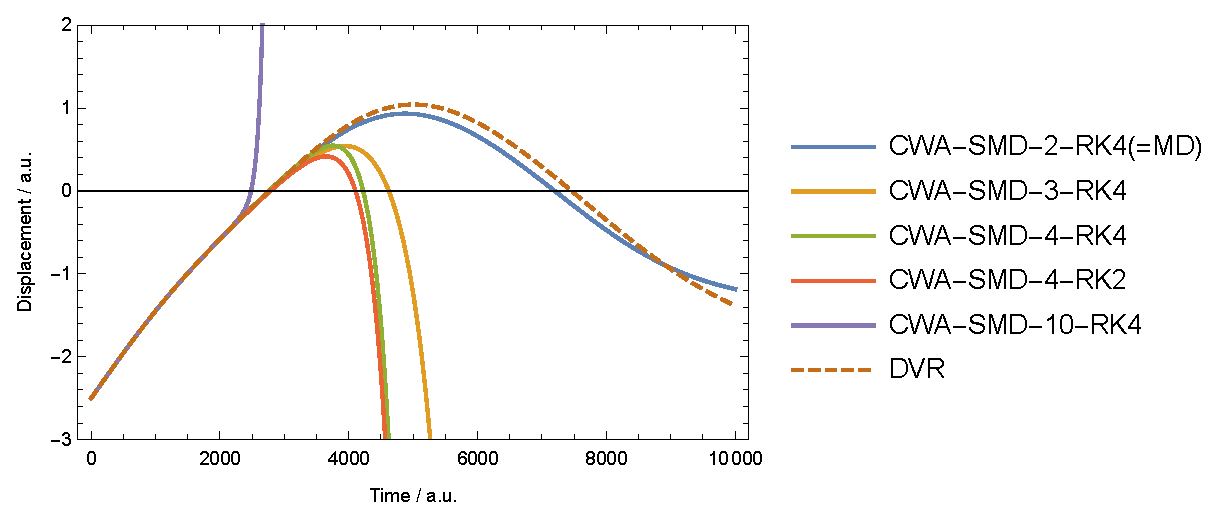
\includegraphics[width=0.8\textwidth]{cwa_smd.eps}
\caption{双势阱模型中CWA-SMD方法的演化结果与DVR、CWA的对照}
\label{cwa-smd-double-well}
\end{figure}
其典型结果如图 \ref{cwa-smd-double-well}所示。其中,CWA-SMD后的数字代表了追踪的可观察量的最高阶数,而更高阶的可观察量的期望值由CWA近似提供。作为示例,CWA-SMD-5只追踪1至5阶的可观察量的期望值(如 $x$, $p^2$, $x^2 p^3$等)。可以明显看出,高于2阶的CWA-SMD方法都在3000 a.u.附近与精确解(DVR)发生偏离,同时误差不断累积直至发生绝对性的偏差。而CWA-SMD-2的结果与CWA方法一致的原因是不高于2阶的可观察量($x, p, xp, x^2, p^2$)在磨雅括号下给出的演化方程与经典力学中的泊松方程一致(因为不存在三阶及以上的偏导,对应的项不贡献)。而CWA的演化过程只考虑经典力学部分,因此CWA方法与CWA-SMD-2方法事实上会给出相同的结果。

\begin{figure}
\centering
\subfigure[绝对误差]{
	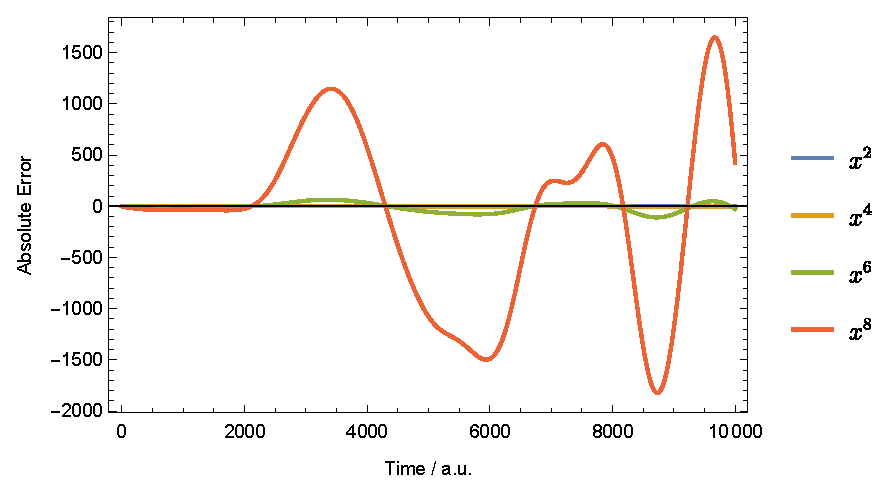
\includegraphics[width=0.46\textwidth]{cwa_exp_absolute_error.eps}	
}
\subfigure[绝对误差]{
	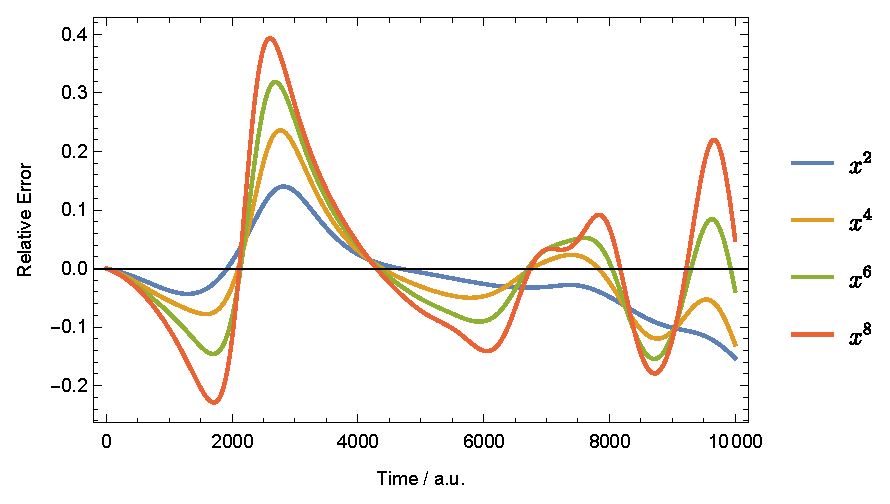
\includegraphics[width=0.46\textwidth]{cwa_exp_relative_error.eps}	
}
\caption{双势阱模型中CWA方法给出的一些典型的可观察量的期望值与DVR方法的差异}
\label{exp-error}
\end{figure}
为研究CWA-SMD方法产生的误差的来源,我们考察了在该模型下DVR方法与CWA方法在高阶可观察量下的期望值的差异,如图 \ref{exp-error}所示。

我们同时考察了非谐性振子模型,其


\begin{figure}
\centering
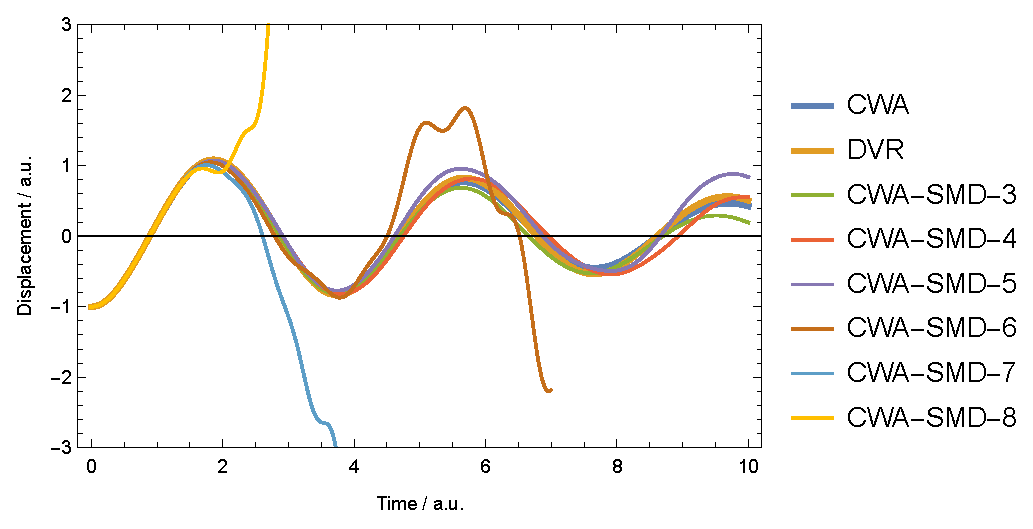
\includegraphics[width=0.8\textwidth]{anharmonic_cwa_smd.eps}
\caption{非谐性振子模型中CWA-SMD方法的演化结果与DVR、CWA的对照}
\label{cwa-smd-double-well}
\end{figure}

\begin{figure}
\centering
\subfigure[绝对误差]{
	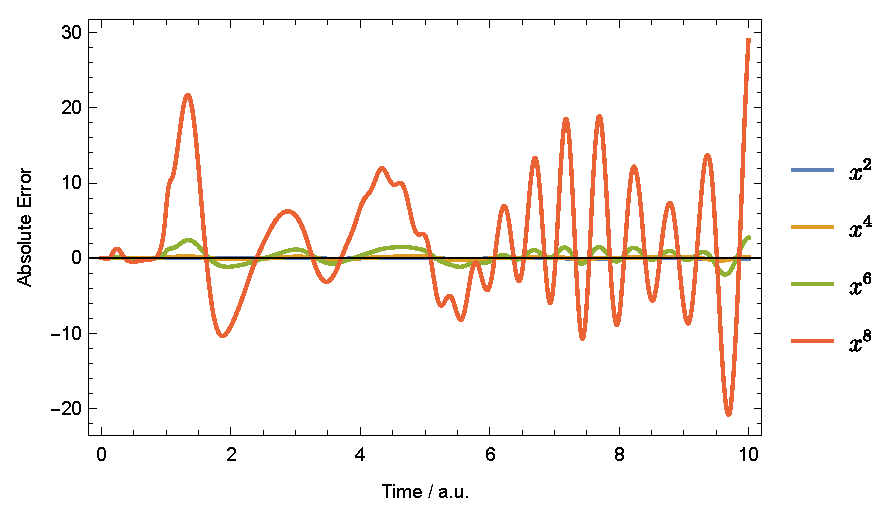
\includegraphics[width=0.46\textwidth]{cwa_exp_absolute_error_anharmonic.eps}	
}
\subfigure[绝对误差]{
	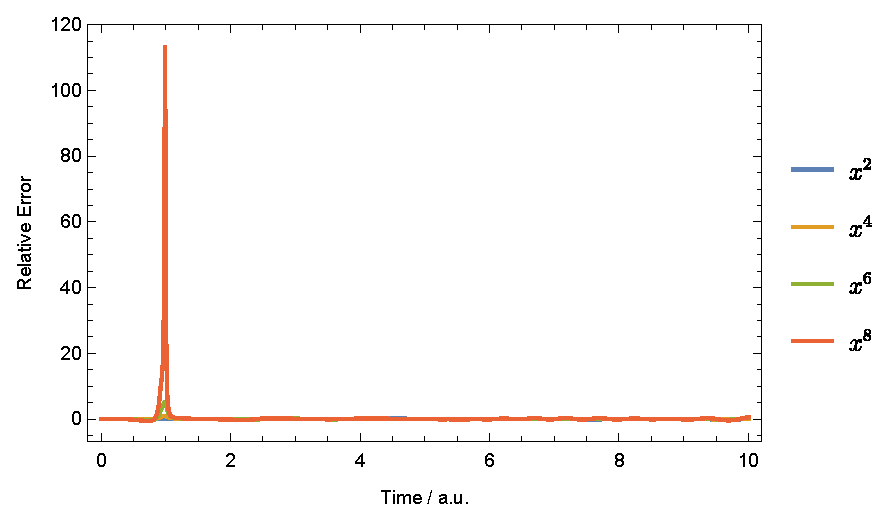
\includegraphics[width=0.46\textwidth]{cwa_exp_relative_error_anharmonic.eps}	
}
\caption{非谐性振子模型中CWA方法给出的一些典型的可观察量的期望值与DVR方法的差异}
\label{exp-error-anharmonic}
\end{figure}
